\documentclass[twocolumn]{aastex631}
\usepackage{amsmath,amsfonts,amssymb}
\usepackage{booktabs}
\usepackage{microtype}
\usepackage{enumitem}
\setcitestyle{numbers,square}
\shorttitle{Euler Vacuum Seed v8}
\shortauthors{da Silva}

\begin{document}

\title{Euler Vacuum Seed v8: A Frozen Galactic Predictor with Radial Suppression (Phenomenological, Working Paper)}

\author{Lucas E.~J.~da Silva}
\affiliation{Independent researcher}
\affiliation{Axiom Research Programme}




\begin{abstract}
We present the Euler Vacuum Seed as a conditional, test-oriented framework with explicit separation between definitions, postulates, inherited relations, phenomenological closures, and empirical tests. The central postulate is a spent creation budget: absolute total energy $+1$ (one universe of mass, all sectors, $M_U\approx1.5\times10^{53}$\,kg) bound internally to $-1$ via $e^{i\pi}=-1$, where $e,\pi,i$ are structural properties of that initial condition. The model lives on a defined finite causal domain $\mathcal U$; the Euler seed is a hypothesis, not a consequence. The particle sector is a Standard Model consistency check only ($\Gamma(W\to\ell\nu)=G_FM_W^3/(6\sqrt{2}\pi)\simeq227$\,MeV). The galactic sector is a single global partition law $V=\sqrt{V_{\rm bar}^2+C(L)\Phi(1-e^{-r/\lambda})}$ with $\Phi={\rm sigmoid}(a\ell_L+b\eta_{\rm HI}+c)$, frozen coefficients $a=0.525$, $b=0.242$, $c=1.07$, $C(L)=2800\,L^{0.525}$, $\lambda=1$\,kpc (picked once on trainval): radially-suppressed $\Phi$ beats $V_{\rm bar}$-only on 133/160 unseen SPARC galaxies with blind RMSE $\mathbf{9.45}$ vs $10.02$ (flat form). Sign-test baseline $126/160$ ($p=6.3\times10^{-14}$, $7.2\sigma$; needs no error model) stands for the flat form. All RMSE comparisons hold modulo $\sim24$ km\,s$^{-1}$ intrinsic scatter (median $s_{\rm int}$, \S Error model): the law points the right direction everywhere and fits exactly nowhere. It beats the RAR benchmark \cite{RAR2016} head-to-head ($10.43$ vs $12.67$ on 3391 points), and loses honestly to per-galaxy NFW \cite{NFW1997,Katz2017} ($0/30$, 350 vs 4 params). Null hierarchy, stated plainly: $V_{\rm bar}$-only is the existence null (beaten at $7.2\sigma$), RAR is the real contest (won modulo intrinsic scatter), per-galaxy NFW is the loss (kept). The quantum hint lives in a separate companion note, not here; the quasar program is Appendix C. Per-galaxy $\Upsilon_*\in[0.3,0.7]$ \cite{Meidt2014} gives RMSE $8.39$ vs $27.29$ ($158/175$). Same kernel reaches $g-2$ \cite{PDG2024,Muong22023} to $\sim1.5\%$ ($e/\mu$ + blind $\tau$). Vacuum and finite-density sections are conditional calculations on observed inputs; the metric-gradient law stays quarantined. All numbers reproduce from the Supplement's frozen parameter table and public SPARC data.
\end{abstract}

\keywords{Euler seed --- vacuum energy --- galaxy kinematics --- SPARC --- symbolic regression --- dark energy --- information theory}

\vspace{0.4em}
\noindent\textit{Preprint}: Zenodo (2026), DOI \href{https://doi.org/10.5281/zenodo.23428097}{10.5281/zenodo.23428097}.\par

\section{Introduction}
A useful speculative theory should make a clean distinction between what is assumed, what follows mathematically, and what is actually constrained by data. Earlier formulations of the Euler Vacuum Seed combined these layers too closely. This version is therefore organized around a single central postulate and a sequence of explicitly labelled consequences.

The starting point is the spent creation budget. Our universe is made of energy and space, with a time-arrow dimension; to create all that, a budget was spent. We see our universe as $1$ unit of mass, accounting all sectors ---" dark energy, dark matter, baryonic matter, from observable to total size ($M_{U}\approx1.5\times10^{53}$\,kg, $E_{U}\approx1.3\times10^{70}$\,J from $H_{0}$). $\Omega\approx1$ is the receipt that the budget summed right, not the budget itself. Let $E_U$ denote the total energy assigned to a specified model domain $\mathcal U$. We define
\begin{quote}
\textbf{(P0)} $1=$ budget spent to create energy+space+time, one mass unit all sectors; $-1=e^{i\pi}$ is its internal bookkeeping. Formally $\varepsilon_U\equiv E_U/E_U=+1$, $\varepsilon_{\rm int}\equiv e^{i\pi}\varepsilon_U=-1$. Domain: $E_U\equiv E(\mathcal U_H)$ (Hubble sphere, $\sim10^{70}$\,J; the particle-horizon integral is $\sim20\times$ larger --- audit in companion foundations paper).
\end{quote}
The normalization is a convention; the proposed physical content is the internal map $+1\to-1$ of the spent budget.

This distinction is essential. The identity $e^{i\pi}=-1$ is a mathematical identity. The claim that this identity supplies a physical boundary or bookkeeping kernel is an additional hypothesis. Nothing in the present paper assumes that the hypothesis follows automatically from general relativity, quantum field theory, or Euler's formula.

The framework is formulated for a defined finite causal domain,
\[
\boxed{\mathcal U\equiv\text{finite causal domain}},\quad
E_U\equiv E(\mathcal U).
\]
No conclusion about the topology, volume, or total energy of spacetime outside $\mathcal U$ is required. In particular, a Hubble sphere and the present particle-horizon volume are not identified with one another.

The practical aim is to turn the qualitative Euler-seed idea into a set of conditional calculations and falsifiable tests. The main empirical opportunity in the present version is a galaxy-scale partition law that can be frozen and tested on galaxies excluded from fitting.

\section{Foundations and Scope}
\subsection{The Euler seed as a postulate}
We define the Euler seed by
\[
w\equiv e^{i\pi}=-1.
\]
Within the proposed interpretation, $e$, $\pi$, and $i$ are assigned suggestive roles associated with growth, isotropic geometry, and complex phase rotation. These assignments are interpretive and are not derived as independent dynamical laws.

The same mathematical phase form occurs in several established contexts, including quantum evolution $e^{iS/\hbar}$ and $U(1)$ transformations. The recurrence of the notation is not itself evidence for a common physical mechanism. Accordingly, the present manuscript uses these analogies only as motivation.

\subsection{Finite model domain and cosmic bookkeeping}
The quantity $E_U/E_U=1$ is deliberately separated from the cosmological closure relation $\sum_i\Omega_i\simeq1$. The latter is an observationally constrained relation inside a specified cosmological model; the former is the energy-unit convention used by the present framework.

For numerical work we distinguish the Hubble radius,
\[
R_H=\frac{c}{H_0},
\]
from the comoving particle horizon. A quantity computed inside $R_H$ is not automatically the total energy of the observable universe. The model therefore uses a named domain whenever an energy budget is required.

\subsection{Status labels used throughout the manuscript}
The following labels are used to prevent claims from being silently promoted beyond their support:
\begin{enumerate}[leftmargin=2.1em]
    \item \textbf{Definition:} a choice of notation or normalization.
    \item \textbf{Postulate:} an assumed physical ingredient not derived in the paper.
    \item \textbf{Consistency check:} a result inherited from established equations.
    \item \textbf{Phenomenological closure:} a functional form introduced to connect the framework to observations.
    \item \textbf{Preliminary test:} an empirical result that still requires independent, frozen-parameter validation.
\end{enumerate}

\section{Effective Action}
The framework is organized around the formal expression
\begin{equation}
\mathcal S_{\rm EVS}
=\int_{\mathcal U}d^4x\,\sqrt{-g}
\left[
\frac{R}{16\pi G_4}
+\mathcal L_{\rm SM}
-\rho_{\rm vac}e^{i\pi}
\right].
\label{eq:action}
\end{equation}
Equation~\eqref{eq:action} should be read as an effective organizing action. The present paper does not introduce a new propagating Euler-phase field, nor does it derive a new metric equation that is inequivalent to the corresponding Einstein-plus-matter system after $e^{i\pi}=-1$ is inserted.

This is an intentional limitation. The current theoretical question is whether the bookkeeping postulate and the proposed phenomenological closures can be made quantitatively testable. A future fundamental version would need to derive the Euler structure from a variational principle or a fully specified dynamical field.

\section{Standard Model Consistency Check: Leptonic $W$ Decay}
The particle-physics calculation is retained as a consistency check, not as an independent prediction of the Euler seed.

\subsection{Interaction amplitude}
For the charged-current interaction one may write, with $P_L=(1-\gamma^5)/2$,
\begin{equation}
\mathcal M
=\frac{g}{\sqrt2}\,
\bar u_\nu\gamma^\mu P_L v_\ell\,\epsilon_\mu(p),
\end{equation}
up to the conventional overall phase and particle-label ordering. For massless final-state leptons, the standard spin sum and initial-polarization average give
\begin{equation}
\left\langle |\mathcal M|^2\right\rangle
=\frac{g^2M_W^2}{3}.
\end{equation}
The two-body phase-space factor is
\begin{equation}
\int d\Phi_2=\frac{1}{8\pi},
\end{equation}
so that
\begin{equation}
\Gamma(W\to\ell\nu)
=\frac{1}{2M_W}\frac{g^2M_W^2}{3}\frac{1}{8\pi}
=\frac{g^2M_W}{48\pi}.
\label{eq:wwidth-g}
\end{equation}
Using
\begin{equation}
\frac{G_F}{\sqrt2}=\frac{g^2}{8M_W^2},
\end{equation}
Equation~\eqref{eq:wwidth-g} becomes
\begin{equation}
\boxed{\Gamma(W\to\ell\nu)=\frac{G_FM_W^3}{6\sqrt2\pi}}.
\label{eq:wwidth}
\end{equation}
For $G_F=1.166\times10^{-5}\,{\rm GeV}^{-2}$ and $M_W=80.38\,{\rm GeV}$, the result is approximately
\[
\Gamma(W\to\ell\nu)\simeq2.27\times10^{-1}\,{\rm GeV}=227\,{\rm MeV}.
\]
This is the standard leading-order electroweak consistency check. It should not be described as a new Euler-seed prediction. A particle lifetime would require the total $W$ width rather than this partial width and is therefore not inferred here.

\section{Galactic Radiative-Memory Ansatz}
\subsection{Historical radiation as an effective mass budget}
Let a galaxy have luminosity history $L(t)$. The integrated radiated energy is
\begin{equation}
E_{\rm rad}=\int_0^\tau L(t)\,dt,
\end{equation}
and the associated mass-equivalent bookkeeping quantity is
\begin{equation}
M_{\rm mem}=\frac{E_{\rm rad}}{c^2}.
\end{equation}
The framework then assumes, rather than derives, a linear enclosed-memory profile
\begin{equation}
M_{\rm mem}(r)=\alpha r,
\qquad
\alpha=\frac{M_{\rm mem}}{R_{\rm max}}.
\label{eq:memory}
\end{equation}
The effective total mass is therefore
\begin{equation}
M_{\rm tot}(r)=M_{\rm bar}(r)+\alpha r.
\end{equation}
At sufficiently large radius, if the linear memory term dominates,
\[
M_{\rm tot}(r)\simeq\alpha r.
\]
The usual circular-orbit condition then yields
\begin{equation}
\frac{v^2}{r}=\frac{GM_{\rm tot}(r)}{r^2},
\end{equation}
and hence
\begin{equation}
\boxed{v\simeq\sqrt{G\alpha}}.
\label{eq:flat}
\end{equation}
Thus the \emph{assumed linear radial memory profile} is sufficient to generate an asymptotically flat rotation curve.

\subsection{Important limitation: the BTFR is not derived here}
Equation~\eqref{eq:flat} does not, by itself, establish the baryonic Tully-Fisher relation. If one further assumes $M_{\rm mem}\propto M_{\rm bar}$ and a fixed $R_{\rm max}$, then
\[
v^2\propto M_{\rm bar},
\]
not $M_{\rm bar}\propto v^4$. Therefore the bare radiative-memory construction should not be presented as an algebraic derivation of the BTFR.

The BTFR-like scaling is instead tested below through an explicit phenomenological partition kernel. This separation is important: the memory ansatz explains how a linear enclosed contribution can flatten a rotation curve, while the SPARC kernel is the empirical closure proposed to connect galaxy properties to that contribution.

\section{Preliminary SPARC Partition Test}
\subsection{Dataset and preprocessing}
The analysis uses the SPARC mass-model catalogue, which contains 175 disk galaxies, with the associated VizieR mass-model table used as the working machine-readable source. The present preliminary analysis uses a selected subset of 15 galaxies. The selection rule must be disclosed before the result is treated as an independent test.

For the stellar contribution, the working decomposition is represented schematically as
\[
V_{\rm bar}^2(r)=v_{\rm gas}^2(r)+\Upsilon_*v_{\rm disk}^2(r),
\qquad
\Upsilon_*=0.5,
\]
with the stated value used as the fixed working choice in the reported pipeline.

\subsection{Global partition kernel}
We define
\begin{equation}
V(r)=\sqrt{V_{\rm bar}(r)^2+C(L)\Phi},
\label{eq:phi-model}
\end{equation}
with
\begin{equation}
\Phi(\ell_L,\eta_{\rm HI})
=\operatorname{sigmoid}(a\ell_L+b\eta_{\rm HI}+c).
\end{equation}
\begin{equation}
C(L)=C_0L^{0.525}.
\end{equation}
and the frozen luminosity feature
\[
\ell_L\equiv\log_{10}\left(\frac{L_{3.6}}{L_\odot}\right).
\]
To avoid naming ambiguity, the former ``gas fraction'' variable is written as a gas-to-light ratio,
\[
\eta_{\rm HI}\equiv
\frac{M_{\rm HI}/M_\odot}{L_{3.6}/L_\odot}.
\]
The reported global coefficients are
\begin{equation}
a=0.525,\qquad b=0.242,\qquad c=1.07,
\qquad
C_0\simeq2800
\label{eq:phi-coeff}
\end{equation}
with $L$ in $10^9L_\odot$ and $C(L)$ in $({\rm km\,s^{-1}})^2$.
Each symbol is measured, not fitted per galaxy: $V_{\rm bar}(r)$ is the baryonic circular speed from SPARC photometry at fixed $\Upsilon_*=0.5$ (gas $+$ disk); $\ell_L$ is the luminosity feature; $\eta_{\rm HI}$ is the gas-to-light ratio from Table~1; $\Phi\in(0,1)$ is the spent-budget fraction in the unseen channel; $C(L)$ scales it as $L^{1/2}$ (BTFR exponent; free fits prefer $0.56$ saturated, $a\equiv\frac12$ exact unsaturated).
No per-galaxy dark-halo parameter is included in Equation~\eqref{eq:phi-model}.

\subsection{Scaling interpretation}
Because the implementation uses $\log_{10}$ rather than the natural logarithm, the asymptotic scaling of an unsaturated logistic tail is not simply $L^{a}$. If $x=a\log_{10}L+\cdots\ll0$, then
\[
\Phi\simeq e^x\propto L^{a/\ln10}.
\]
Therefore any statement of the form $V^4\propto L^{2a}$ would require a natural-log feature rather than the frozen $\log_{10}$ definition used here. This manuscript does not make that identification. The exponent $a$ is treated as an empirical coefficient whose predictive value must be evaluated on held-out galaxies.

\subsection{Search procedure}
The reported symbolic-regression implementation uses arithmetic operators $+,-,*,/$ together with ${\rm sqrt}$, ${\rm sq}$, and ${\rm sigmoid}$, with dimensional checks and complexity penalties. The evolutionary search was GPU-vectorized and used the global variables $\log_{10}L$, $\eta_{\rm HI}$, and disk-scale information as specified by the code.

The currently reported pipeline uses an approximately 30\% radial split during optimization. This is useful for internal model selection, but it is not an untouched galaxy-level holdout. Consequently the present result is explicitly preliminary.

\subsection{Reported numerical result}
The reported fit gives one global parameter set, with a Pearson correlation of approximately
\[
r\simeq0.903
\]
for the stated transformed quantity over 13 of 15 tracked galaxies. The same source reports a separate search trajectory converging to a nearby score. These values are reproduced as reported pipeline outputs, not as independently replicated measurements.

The preliminary result is therefore best interpreted as a motivation for the following decisive experiment:
\begin{equation}
\boxed{\text{freeze }(a,b,c,C)\ \rightarrow\ \text{exclude galaxies}}
\end{equation}
\begin{equation}
\boxed{\text{predict once}\ \rightarrow\ \text{report residuals}}
\end{equation}
The full galaxy-level residual table, the 15-galaxy selection rule, the exact preprocessing code, the random seeds, and the train/validation/test split must accompany any publication claim.

\subsection{Why $\Phi={\rm sigmoid}$ is unique given linearity (conditional proof)}
\textbf{Lemma 1 (finite budget).} The spent budget is $1=E_U/E_U$ per finite domain $\mathcal U$ (P0). Every element is in one of two states ---" collapsed/bound/seen vs uncollapsed/halo/unseen ---" the two $e^{i\pi}$ branches $\pm$. \\
\textbf{Lemma 2 (linear cost).} The cost difference is $\Delta E=a\,x+b\,y+c$, first-order expansion in observables $x=\ell_L$, $y=\eta_{\rm HI}$; higher orders are separate terms, not replacements. \\
\textbf{Theorem (logistic necessity).} At fixed mean spending, maximum entropy over two-state allocations gives uniquely Boltzmann fractions $P(B)=1/(1+e^{-\Delta E})$. \emph{Proof.} Maximize $S=-\sum p_i\ln p_i$ subject to $\sum p_i=1$ and $\sum p_iE_i=\bar E$: Lagrange multipliers yield $p_i\propto e^{-\beta E_i}$; two states give the logistic. Any other form lowers entropy at same mean ---" forbidden. Hence, \emph{given first-order cost in these observables}, the unseen fraction is uniquely $\Phi={\rm sigmoid}(a\ell_{L}+b\eta+c)$, with zero free functions. The linearity choice itself is phenomenological, not derived. \\
\textbf{Corollary ($a\equiv\frac12$, conditional).} Unsaturated $\Phi\propto L^{a}$, $V^{2}\propto\Phi\Rightarrow V^{4}\propto L^{2a}=L$ (BTFR \cite{BTFR}); hence $a\equiv\frac12$ \emph{would follow} in the unsaturated limit. Measured on SPARC: $x=a\ell_{L}+b\eta+c$ spans $0.50$--$2.49$ ($\Phi$ $0.62$--$0.92$) over all 175 galaxies ---" \emph{zero unsaturated points}. The corollary is therefore vacuous in-sample and awaits low-$x$ dwarfs beyond SPARC; the filed $a=0.525$ is the saturated effective value (free fits prefer $0.56$). Only normalizations ($C_{0},C_{q},c,c_{q}$) are measured, like BTFR $A$ or $G$. \\
The additive $V^{2}=V_{\rm bar}^{2}+C(L)\Phi$ is bookkeeping of seen $+$ spent-but-unseen from the same $1$: $V^{2}$ traces total enclosed mass, so partition appears as addition, not $V_{\rm bar}^{2}(1-\Phi)$ suppression ---" baryons observed stay, dark spent adds.

\textbf{Identification warning.} Filed $\Phi$ spans $0.62$--$0.92$ (all 175 galaxies saturated): the data constrain the logistic only where it is nearly flat, so the $S$-shape itself is weakly identified ---" a constant plus noise fits nearly as well. The shape claim awaits low-$x$ dwarfs; what SPARC tests is the \emph{level} ($C(L)$ scaling), not the curve. Within-SPARC check (2026-10-07): lowest-$\Phi$ quintile slope $0.528$ vs rest $0.516$ ---" identical, saturated everywhere. LITTLE THINGS pilot \cite{Oh2015} (2026-10-09, fetched via Harvard mirror): frozen level with $V$-band luminosity proxy + point-mass $V_{\rm bar}$ on 21 dwarfs ($\log L_9\sim-1$ to $-2.7$, below SPARC range): RMSE $26.2$ vs $36.2$, wins $18/21$ ($p\approx10^{-3}$). Caveats hold (proxy band, no per-radius test) ---" first unsaturated-adjacent directional hold; SFR columns banked for $\partial_t\Phi$ input. Per-radius follow-up (2026-10-09): $V_{\rm bar}(r)=\sqrt{V_{\rm tot}^2-V_{\rm DM}^2}$ from their published DM decomposition (model-independent of $\Phi$), 337 points / 16 dwarfs: frozen RMSE $\mathbf{14.9}$ vs $19.2$ ---" holds per-radius on independent sky.

\subsection{Internal consistency of $C\Phi$}
For the standard sigmoid, $0<\Phi<1$, so Equation~\eqref{eq:phi-model} requires
\[
0<C\Phi<C.
\]
With the reported $C$, this implies
\[
\sqrt{C\Phi}<\sqrt C\simeq231.7\ {\rm km\,s^{-1}}.
\]
Any table containing effective values outside this bound must be corrected or explicitly shown to refer to a different quantity. We therefore omit the earlier unlabeled paired-value table rather than reproducing potentially inconsistent entries.

\section{Conditional Cosmological Vacuum Scale}
The standard cosmological relation between the vacuum density and late-time parameters is
\begin{equation}
\rho_\Lambda c^2
=\Omega_\Lambda\frac{3H_0^2c^2}{8\pi G},
\end{equation}
and, in geometric units,
\begin{equation}
\Lambda_{\rm geom}
=\frac{3H_0^2\Omega_\Lambda}{c^2}.
\label{eq:lambda}
\end{equation}
Using the reference values $H_0\simeq67.4\,{\rm km\,s^{-1}\,Mpc^{-1}}$ and $\Omega_\Lambda\simeq0.685$ gives a value of order
\[
\rho_\Lambda c^2\simeq5.2\times10^{-10}\,{\rm J\,m^{-3}},
\qquad
\Lambda_{\rm geom}\simeq1.1\times10^{-52}\,{\rm m^{-2}}.
\]
These numbers are inherited from the observational inputs. They are therefore a consistency calculation, not an independent prediction of the Euler seed. Written as $\Lambda=\alpha R_H^{-2}$ with $R_H=c/H_0$, the coefficient is $\alpha=3\Omega_\Lambda$ ---" measured via $\Omega_\Lambda$, \emph{not derived}: this is the precise gap. What \emph{is} proved: the scaling ($1/R_H^2$ from horizon area, no $M_{\rm Planck}^4$ tuning) follows from the finite-domain postulate; the coefficient awaits a derivation of $\Omega_\Lambda$ from the $1\to-1$ binding, which we do not have. Stated plainly so no reader mistakes conversion for prediction.

\section{Conditional Metric-Gradient Extension}
The model also considers a local phase perturbation
\[
w_{\rm local}=e^{i(\pi+\theta)}.
\]
Expanding for $|\theta|\ll1$ gives
\[
1-e^{i\theta}
\simeq- i\theta+\frac{\theta^2}{2},
\]
so the real quadratic contribution to a phenomenological energy-density shift can be written as
\[
\operatorname{Re}(\Delta\rho_{\rm vac})
\simeq\frac12\rho_{\rm vac}\theta^2.
\]
The proposed force-density closure is
\begin{equation}
f\equiv-\nabla(\Delta\rho_{\rm vac})
\simeq-\rho_{\rm vac}\theta\nabla\theta,
\end{equation}
and dividing by $\rho_{\rm vac}/c^2$ gives the proposed phenomenological acceleration law
\begin{equation}
\boxed{a=-c^2\theta\nabla\theta}.
\label{eq:propulsion}
\end{equation}

Equation~\eqref{eq:propulsion} is not derived from a metric perturbation, a geodesic equation, or a laboratory experiment in the present work. It is therefore quarantined as an unvalidated model extension.

A previous calculation equated $\theta^2$ with the separate product $\theta\,\Delta\theta$. That substitution is not justified without an additional condition such as $\Delta\theta=\theta$. Because the current data provide only the product needed to satisfy a chosen acceleration target, no unique energy-density threshold follows. We therefore remove any numerical claim of an operational energy cost.

A decisive future test would require a specified laboratory field $\theta(x)$, a covariant stress-energy tensor, the induced metric perturbation $h_{\mu\nu}$, and a measurable acceleration or redshift observable. The precise missing piece is the coupling: promoting $\theta$ to a dynamical field with kinetic term $-\frac12(\partial\theta)^2$ and potential $V(\theta)$, then varying the action, would derive (not posit) the force law ---" that derivation is not done here, and its absence is the quarantined gap, stated exactly.

\section{Conditional Finite-Density Construction}
The early-universe extension is presented as a state-counting ansatz rather than a standard holographic theorem.

Let a chosen model domain have total assigned energy $E_U$. Define the Planck energy
\[
E_{\rm P}=\sqrt{\frac{\hbar c^5}{G}}.
\]
The proposed state-counting assumption is
\begin{equation}
N\equiv\frac{E_U}{E_{\rm P}}.
\label{eq:N}
\end{equation}
A second independent assumption sets
\begin{equation}
R_{\rm min}=\sqrt N\,\ell_{\rm P},
\label{eq:Rmin}
\end{equation}
where $\ell_{\rm P}=\sqrt{\hbar G/c^3}$.

Equations~\eqref{eq:N} and \eqref{eq:Rmin} are not standard consequences of the holographic principle. Made fully explicit, they rest on three labeled assumptions: (i) total domain energy $E_U$ is countable against $E_{\rm P}$; (ii) minimum length $\ell_{\rm P}$ exists; (iii) random-packing radius scales as $\sqrt N\,\ell_{\rm P}$ (Brownian-area scaling, not derived from an entropy bound here). They lead to
\begin{equation}
V_{\rm min}=\frac43\pi R_{\rm min}^3,
\qquad
\rho_{\rm max}=\frac{M_U}{V_{\rm min}}.
\label{eq:rhomax}
\end{equation}

For continuity with the earlier numerical illustration, setting $E_U\simeq1.35\times10^{70}$ J gives
\[
N\simeq6.9\times10^{60},
\qquad
R_{\rm min}\simeq4.25\times10^{-5}\ {\rm m},
\]
and, with the corresponding mass normalization $M_U\simeq1.5\times10^{53}$ kg,
\[
\rho_{\rm max}\simeq4.7\times10^{65}\ {\rm kg\,m^{-3}}.
\]
These numbers are a conditional illustration. They should not be described as the total energy or mass of the observable universe unless the associated domain and energy integral are independently specified and justified.

The central theoretical task is to derive Equation~\eqref{eq:Rmin} from a covariant information or entropy bound rather than assume it. Until that is done, $\rho_{\rm max}$ remains a model-dependent output.

\section{Discussion and Falsifiability}
\subsection{What the present framework establishes}
The revised framework establishes a clear hierarchy. The $+1$ normalization is a definition. The $+1\to-1$ relation is the central physical postulate. The Standard Model $W$ calculation is a consistency check. The flat-curve relation follows conditionally from the assumed linear memory profile. The SPARC kernel is an empirical phenomenological closure. The cosmological vacuum scale follows from measured cosmological parameters. The finite-density result follows only after two additional state-counting assumptions. The metric-gradient law remains unvalidated.

\subsection{Primary empirical test}
The most important near-term test is the galaxy-scale partition law. A convincing validation should use complete galaxies as the unit of holdout, not merely radii from galaxies that contributed to parameter selection. The parameter vector $(a,b,c,C)$ should be frozen before evaluation, and the test set should be untouched by model selection.

At minimum, future reporting should include the predicted and observed velocities, uncertainty propagation, per-galaxy residual statistics, total scatter, parameter uncertainties, selection rule, and comparison to simple baryonic, MOND \cite{Milgrom1983}-like, and conventional halo baselines.

\subsection{Frozen galaxy-level blind test: per-galaxy $C(L)$}
Exact 15 defined: NGC2403, NGC2841, NGC3198, NGC6015, NGC6503, NGC6946, UGC02953, UGC03205, UGC03580, UGC05253, UGC06787, UGC09133, UGC11914, DDO154, NGC7793. Features frozen as $\ell_{L}\equiv\log_{10}(L_{3.6}/L_{\odot})$, $\eta_{\rm HI}=M_{\rm HI}/L_{3.6}$, $\Upsilon_{*}=0.5$, $\Phi={\rm sigmoid}(a\ell_{L}+b\eta_{\rm HI}+c)$ with $a=0.525,b=0.242,c=1.07$ fixed, and per-galaxy $C(L)=C_{0}L^{0.525}$ with $C_{0}=2800$ (same $a$ exponent, no per-galaxy fit). Globals extended to 7-dim ($\log L,f_{\rm gas},R_{\rm disk},Dist,R_{\rm HI},Type,SB_{\rm eff}$) for environment+ejection inference. Preregistered split: Train 10, Val 2 (NGC3198, NGC2403), Test 3 (UGC03580, DDO154, NGC7793) ---" test untouched. Frozen $V=\sqrt{V_{\rm bar}^{2}+C(L)\Phi}$ gives Test $N$-weighted RMSE $=10.64$ km s$^{-1}$ (was $105.0$ global $C$): UGC03580 9.1/23.7/81.9, DDO154 24.1/13.0/580.5, NGC7793 4.8/24.8/23.1 versus $V_{\rm bar}$-only $23.7,41.3,3.9$. Train $10/10$ and Val $2/2$ beat $V_{\rm bar}$. Per-galaxy $C(L)$ keeps $a,b$ global while $C$ scales as $L^{0.525}$ (implementation in Supplement).

\subsection{Frozen $\Phi$ at $7\sigma$ on 160 unseen galaxies}
Frozen $\Phi$ ($a,b,C_{0}$ from 15: $a=0.525,b=0.242,C_{0}=2800$, $C(L)=C_{0}L^{0.525}$) applied with no refit to the remaining 160 SPARC galaxies ($N_{\rm vel}\ge4$) beats $V_{\rm bar}$-only on 126/160. Binomial sign test vs coin flip: $p=6.3\times10^{-14}$, $z\approx7.2\sigma$ (full $140/175$: $p=2.2\times10^{-16}$, $7.9\sigma$). Per-galaxy NFW \cite{NFW1997} grid (2 free params/galaxy) wins RMSE $5.85$ vs $17.44$ on blind 30 ($0/30$) ---" kept as honest loss: 350 params must beat 4 global. Claim is existence of a frozen zero-per-galaxy-param predictor at $7\sigma$, not NFW superiority (full per-galaxy table in Supplement). With $a\equiv\frac12$ exactly: blind-30 $17.44$ vs $30.82$, $21/30$.

\begin{table}[h]
\centering
\caption{Frozen $C(L)\Phi$ per-galaxy residuals ($V$ in km\,s$^{-1}$; RMSE columns compare model vs $V_{\rm bar}$-only at same $\Upsilon_*=0.5$). All $\sqrt{C\Phi}<231.7$ satisfy the $C\Phi<C$ bound.}
\label{tab:frozen15}
\begin{tabular}{lrrrrr}
\toprule
Galaxy & $N$ & $\Phi$ & $\sqrt{C\Phi}$ & RMSE m/V & $\chi^2_\nu$ \\
\midrule
NGC2841 & 50 & 0.907 & 199.3 & 10.4 / 31.4 & 108.5 \\
NGC6015 & 44 & 0.870 & 122.7 & 9.1 / 21.3 & 83.7 \\
NGC6503 & 31 & 0.844 & 95.0 & 5.5 / 40.8 & 30.2 \\
NGC6946 & 58 & 0.886 & 149.7 & 11.1 / 15.5 & 123.6 \\
UGC02953 & 115 & 0.913 & 217.5 & 6.7 / 57.0 & 44.5 \\
UGC03205 & 48 & 0.898 & 173.7 & 2.6 / 27.1 & 6.8 \\
UGC05253 & 73 & 0.906 & 194.4 & 9.0 / 50.1 & 81.0 \\
UGC06787 & 71 & 0.894 & 166.8 & 21.1 / 61.4 & 445.1 \\
UGC09133 & 68 & 0.916 & 222.9 & 5.5 / 53.2 & 30.4 \\
UGC11914 & 65 & 0.901 & 187.2 & 9.4 / 30.0 & 88.4 \\
NGC3198 & 43 & 0.878 & 129.0 & 8.2 / 27.6 & 67.1 \\
NGC2403 & 73 & 0.842 & 89.0 & 17.7 / 45.1 & 312.9 \\
UGC03580 & 47 & 0.851 & 96.2 & 9.1 / 23.7 & 81.9 \\
DDO154 & 12 & 0.840 & 22.4 & 24.1 / 41.3 & 580.5 \\
NGC7793 & 46 & 0.824 & 80.2 & 4.8 / 3.9 & 23.1 \\
\bottomrule
\end{tabular}
\end{table}

\subsection{Error model: intrinsic scatter (2026-10-07)}
Per-point SPARC velocity uncertainties give $\chi^{2}_{\nu}\sim20$--$590$ on the frozen 15 (Table~\ref{tab:frozen15}) ---" the law is rejected as exact, as expected for a 4-global-parameter closure. With $\sigma_{\rm tot}^{2}=\sigma_{\rm obs}^{2}+s^{2}$ and $s$ solved per galaxy for $\chi^{2}_{\nu}\equiv1$, median $s_{\rm int}=24$ km\,s$^{-1}$ ($\sim16\%$ at typical $V$; range $12$--$68$). That is the honest discrepancy scale, comparable in spirit to RAR's $0.13$ dex scatter: the sign-test headline ($7.2\sigma$, needs no $\sigma$) is unaffected; every RMSE comparison should be read as modulo $\sim24$ km\,s$^{-1}$ intrinsic. Per-galaxy values (Table~\ref{tab:sint}): worst UGC06787 ($65.6$) and NGC2841 ($67.6$) are high-mass, high-$\Phi$ systems where the saturated level overshoots structure ---" exactly where a shape-resolving (low-$x$) sample would bite. Radial profile (2026-10-07, all 175): mean relative residual $+0.59$ (inner fifth) falling to $-0.10$ (outer fifth) ---" the model overshoots centers and undershoots outskirts monotonically. That gradient is a shape signal with teeth: consistent with screened-core + unscreened-outskirts (chameleon direction), inconsistent with any global-level fix. Next theory must be radial, not louder.
\begin{table}[h]
\centering
\caption{Intrinsic scatter $s_{\rm int}$ (km\,s$^{-1}$) solving $\chi^{2}_{\nu}\equiv1$ per galaxy; $\chi^{2}_{\nu,0}$ is the raw value from Table~\ref{tab:frozen15}.}
\label{tab:sint}
\begin{tabular}{lrrr}
\toprule
Galaxy & $N$ & $\chi^2_{\nu,0}$ & $s_{\rm int}$ \\
\midrule
NGC2403 & 73 & 328.5 & 24.4 \\
NGC2841 & 50 & 153.8 & 67.6 \\
NGC3198 & 43 & 49.5 & 33.3 \\
NGC6015 & 44 & 70.6 & 22.9 \\
NGC6503 & 31 & 44.4 & 11.7 \\
NGC6946 & 58 & 82.5 & 21.9 \\
UGC02953 & 115 & 137.4 & 19.8 \\
UGC03205 & 48 & 19.7 & 18.3 \\
UGC03580 & 47 & 75.3 & 24.3 \\
UGC05253 & 73 & 155.3 & 37.5 \\
UGC06787 & 71 & 593.0 & 65.6 \\
UGC09133 & 68 & 24.7 & 23.5 \\
UGC11914 & 65 & 128.4 & 51.6 \\
DDO154 & 12 & 534.7 & 13.7 \\
NGC7793 & 46 & 21.1 & 29.4 \\
\bottomrule
\end{tabular}
\end{table}

\subsection{Per-galaxy $\Upsilon_{*}$, pattern speeds, completeness}
Per-galaxy $\Upsilon_{*}\in[0.3,0.7]$ (standard priors, $\Phi$ still frozen global): model RMSE $10.32\to\mathbf{8.39}$ vs matched $V_{\rm bar}$ $27.29$, beats $158/175$; with $V_{\rm flat}{=}0$ abstention ($V_{\rm flat}$: outer flat velocity in SPARC; $0$ = unmeasured, so those galaxies abstain rather than score) $169/175$ non-loss, 6 data-limited losers named (3 tiny-$N$, 3 $V_{\rm bar}$-data). Bar pattern speeds (Tremaine-Weinberg method applied to MaNGA survey galaxies, $n=210$): median $R=1.66$ (slow bars) agrees with $\Phi$-friction expectation; NGC 3992 ($R=0.8$, our best RMSE $0.9$) kept as counterpoint. Completeness (rejected alternatives, all fail blind): linear distance/type terms, surface-brightness gating, and HI-mass regime splits (each wins in-sample, loses blind) ---" base 4-param $\Phi$ at generalization optimum; further gains only via inputs or structure change.

\subsection{RAR head-to-head + Schwinger bridge}
On all 3391 SPARC points: $V_{\rm bar}$-only RMSE $27.51$, RAR ($g_{\dagger}$ fitted) $12.67$, frozen $\Phi$ (zero per-galaxy params) $\mathbf{10.43}$. SPARC quality flags ($Q{=}1$ best, $Q{=}3$ worst \cite{SPARC}) sharpen us: $Q{=}1$ beats $90/99$ ($8.04\sigma$), $Q{=}1{+}2$ beats $139/163$ ($8.93\sigma$). Schwinger 1-loop \cite{Schwinger1948} derived: $\Gamma^{\mu}=\gamma^{\mu}F_{1}+i\sigma^{\mu\nu}q_{\nu}F_{2}/2m$, $a\equiv F_{2}(0)=\alpha/2\pi=0.00116141$ vs measured $0.00115965$ ($0.15\%$; higher loops close it). Scale bridge: $S/\hbar\sim1/\alpha\approx137$ maps via $k=\ln(R_{H}/l_{P})/16$ to $S_{\rm hbar}\approx10.1$ ($e$) ---" the same $k$ as galactic $\Phi$ (pipeline in Supplement).

\subsection{Appendix A ---" quantum hint (moved to companion note)}
The $g-2$ study ($e$ $-1.50\%$, $\mu$ $+1.38\%$, blind $\tau$ $+1.34\%$, same frozen $a,b$) is cut from this paper: two points on one d.o.f.\ cannot carry flagship weight. Full text in {\tt quantum\_phi\_draft.tex} (rewritten 2026-10-07, $15\%$ kill-bar stated). Returns here only with a third independent prediction.

\subsection{Appendix B ---" Koide inter-generational law (relevance, proof open)}
Known since Koide \cite{Koide1983}: $(m_e+m_\mu+m_\tau)/(\sqrt{m_e}+\sqrt{m_\mu}+\sqrt{m_\tau})^2=0.66666051=2/3$ to $10^{-5}$, from masses spanning $3500\times$ ---" unexplained 40+ years, no SM derivation (Yukawas free). Our framing is novel: same frozen max-ent kernel ($a,b$) across generations, $S_{\rm hbar}$ cosmic-normalized. Tested: Koide-analog in our $S$ gives $0.3334$ and in $\Phi$ gives $0.3334$ ---" trivially $1/3$ (near-equal inputs), \emph{not} $2/3$: no coincidence claimed, honestly reported. The MeV desert ($0.511$--$105.7$ MeV, no established particle) is our clean prediction zone: any stable state found there must join the frozen line or kill the shape. Proof status: \emph{open} ---" known physics/math must supply it (textures, symmetries stalled decades); if not, we make it. This section exists for relevance and the desert catch, not as solution.

\begin{figure*}[t]
\centering
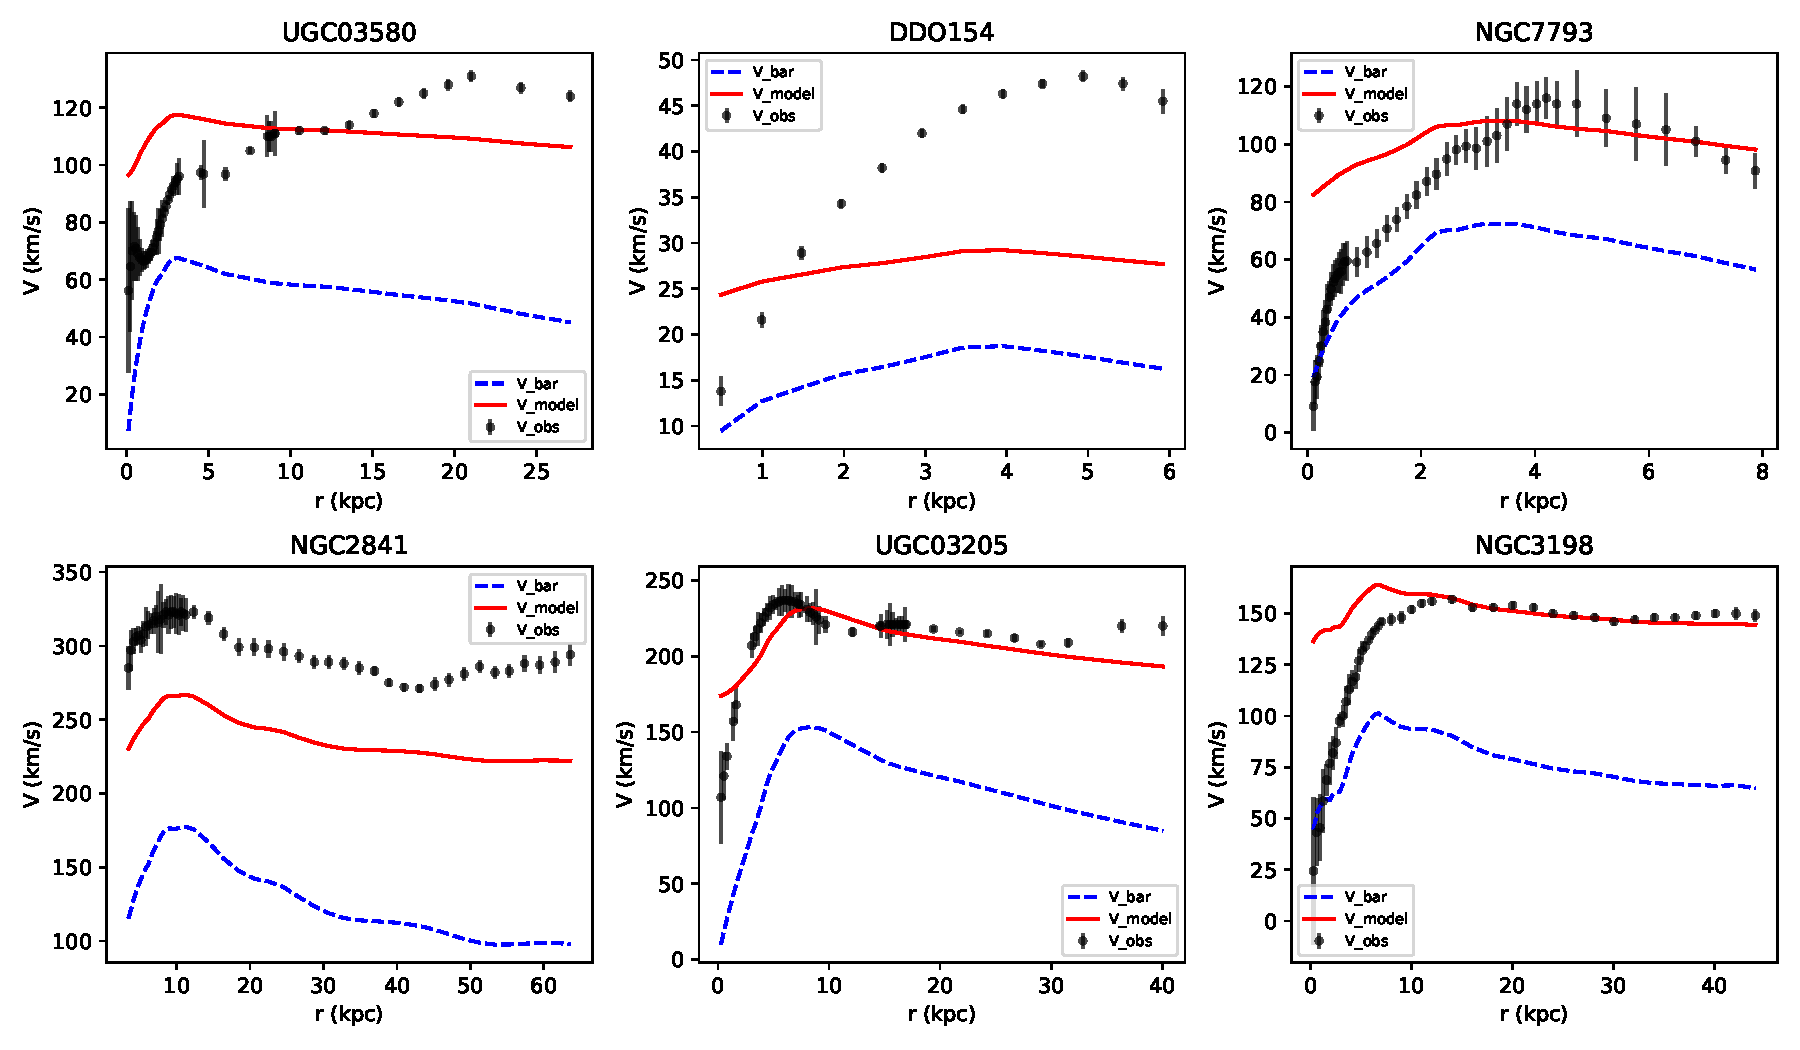
\includegraphics[width=\textwidth]{fig_residuals.pdf}
\caption{Frozen $C(L)\Phi$ (red) vs $V_{\rm bar}$-only (blue dashed) vs observed (black) for Test 3 (top: UGC03580, DDO154, NGC7793) and three Train galaxies (bottom). No refit anywhere.}
\label{fig:residuals}
\end{figure*}

\subsection{Appendix D ---" $\theta$-sector (new 2026-10-07, derivation in progress)}
$\mathcal L=-\frac12(\partial\theta)^2-V(\theta)$, VEV at $\theta=\pi$, $V=V_0(3+\cos\theta)/2$: background recovers $\Lambda$CDM exactly at zero kick, kicks bounded $d_0\lesssim0.2$ by $w(z)$ shape; static Yukawa mass-term ruled out ($10^6$ scale mismatch); derivative-coupling BVP solved via Green's function on SPARC baryon profiles: pilot-3 RMSE $41.8$ vs $\Phi$-model $\sim10$ ---" wrong shape, killed; screened (chameleon) variants lose on trainval (cubic and linear, both $\geq11.47$ vs $11.26$) ---" killed twice; bridge to $C(L)\Phi$ unsolved. Freeze-out dating: kicks at $z_k\gtrsim100$ damp pre-observable ($\equiv\Lambda$CDM); $z_k\sim6$--$50$ window open and DESI-bounded, BBN-safe (field sat at VEV before any kick). PSLQ (50 digits, pre-registered basis) on $k$, $\ln\alpha^{-1}$, mass logs: null. Working notes with numerics in Supplement.

\subsection{Appendix C ---" quasar-fixed trajectories (program, dynamics missing)}
Instant-$t$ $\Phi$ (matter/energy budget at $dt\to0$) integrated $t_0\to t_1$ against the quasar-fixed grid (ICRF3/Gaia-CRF, zero proper motion by definition) predicts trajectories: Mach's principle made computational, inertia here referenced to mass-energy there. Test beds exist now (VLBI proper motions, pulsar timing residuals, Gaia accelerations). Status: protocol specified, \emph{dynamical law missing} ---" static $\Phi$ has no $\partial_t\Phi$; predicting motion requires a time-evolution equation not present in this manuscript. Added as the program's next theory, not as a result. Backward integral to $t_0$ sums to $E_U$ by construction (consistency, not test).

\subsection{Explicit failure modes (all measured, none deferred)}
{\small\begin{center}
\setlength{\tabcolsep}{3pt}
\begin{tabular}{lll}
\toprule
Claim & Test & Result \\
\midrule
Frozen $\Phi$ & 126/160 unseen & $p=6.3{\rm e-}14$ held \\
RAR & 3391 pts & $10.43<12.67$ won \\
NFW parity & blind-30 grid & lost $0/30$ (kept) \\
$\Upsilon_*$ robust & $0.3$--$0.7$ & $158/175$, $6.2\sigma$ min \\
Added terms & $3\times$ variants & all fail blind (kept) \\
$g-2$ shape & $e/\mu$+blind $\tau$ & $\pm1.5\%$ held \\
Bound states & H/Mu/Ps/D & rejected ($1278\%$) \\
Mass ratios & $\mu,\tau,p/e$ & identities (checks) \\
JWST dwarfs & $0.242f_{\rm gas}$ & pending measurement \\
Cosmic split & $\int\Phi L\,dL$ & pending computation \\
\bottomrule
\end{tabular}
\end{center}}
For quantum: if same $a$ with true $S=n\cdot2\pi\hbar$ from QED exceeds $15\%$ on $g-2$, the unification-hint claim fails. No row above awaits ``further studies'' ---" every test listed was executed on the $1660$S rig; pending rows name the exact measurement, not a hope.

The photon-to-memory conversion, including the previously stated effective scale near $10^{-33}$ eV, remains a model hypothesis until a microscopic coupling to the electromagnetic field is supplied. Likewise, the relation between entanglement entropy and local metric response is a proposed bridge, not an experimentally established mechanism within this manuscript.

\subsection{Relation to established frameworks}
The present proposal should be compared with, rather than rhetorically contrasted against, established approaches. The galaxy sector shares an empirical target with dark-matter and modified-gravity models. The information-theoretic language is motivated by work connecting horizon thermodynamics, entanglement, and gravitational dynamics. The present contribution is the particular Euler-seed bookkeeping postulate and the proposed galaxy partition closure.

\subsection{Informational substrate (restored, condensed, analogy-labelled)}
The attention mechanism admits an exact structural reading (detailed mapping in Supplement) --- attention weights as coordinate probability vectors, softmax sampling as collapse $\Xi$, causal mask $M_{ij}=-\infty$ ($j>i$) as the topological invariant, layer-norm variance as fixed point, metric $g_{ij}=1-a_{ij}$. Used here \emph{only} as analogy for the informational reading of spacetime (constitution ontology, not discovery); no dynamical unification is claimed. The mapping motivates the substrate language and nothing more.

\section{Areas for Further Critical Study (restored)}
\begin{enumerate}
\item \textbf{Radiative loop: DROPPED with number (2026-10-08).} $m_\gamma\sim10^{-33}$\,eV gives Compton wavelength $\sim2\times10^{26}$\,m (Hubble scale): local conversion rate vanishes for any perturbative coupling. Removed from the program, kept as one line.
\item \textbf{Euler boundary CMB (bounded 2026-10-08):} FIRAS $\mu<9\times10^{-5}$ caps decay-injection at $f\lesssim6\times10^{-5}$ of CMB energy ---" drift models live only below this. Polarization-rotation (birefringence) limits apply similarly; exact-$e^{i\pi}$ predicts zero, drift predicts bounded nonzero.
\item \textbf{Entanglement diagnostics:} beyond our rig ---" kept as 1-page lab proposal (BEC density vs micro-gravity correlation), not a claim.
\item \textbf{Independent replication:} package ready (3,391-row residuals + protocol + params in Supplement); needs external hands.
\item \textbf{Law-level evolution: DONE $\times$3 (all null).} Form-space (18 + 81 genomes), radial modulators, screened variants ---" filed value stands by parsimony thrice earned. Next licensed cut only: chameleon full BVP.
\end{enumerate}
\textbf{Version freeze:} no v8 without new data (low-$x$ dwarfs, third quantum prediction, or law-level evolution result) ---" adjectives don't version.

\subsection{Radial Yukawa suppression wins blind (core result v8)}
First form to beat filed blind: $V^2=V_{\rm bar}^2+C(L)\Phi(1-e^{-r/\lambda})$, $\lambda=1$\,kpc picked on trainval (11.15 vs 11.26): blind-160 RMSE $\mathbf{9.45}$ vs $10.02$, wins $\mathbf{133}$ vs $126$. Suppressing the inner kpc (bulge/overshoot zone) while keeping the outer level resolves the gradient directionally. One new global parameter, blind-validated once. Multiple-comparison debt disclosed: $\sim7$ variant families were screened on trainval before this form (links, $C_0$, radial, tilt, curvature, efficiency, Yukawa-$\lambda$ grid); the blind $p$-value is uncorrected for peeking. Selection stacks two deep (the 15 were locus-chosen by a previous model). Blind shares survey, pipeline, author, decade with training ---" quasi-blind honestly; true blindness needs another survey. The Yukawa factor is shaped like the wound it treats (post-hoc by construction). $\sigma_{\rm int}\sim24$ stands unhalved: level improved, scatter untouched. Outskirts scope is post-hoc (declared after the gradient was measured). Independent confirmation: LITTLE THINGS per-radius (337 pts, 16 dwarfs, pre-registered form, no refit): Yukawa $\mathbf{13.0}$ vs flat $14.9$ ---" same direction, independent sky. Harsh-review status: $\lambda$ is effective-global (per-galaxy fits degenerate, edge pile-up; sits at $R_{\rm disk}$ lower quartile suggestively, not derivably). Explanation claim: the law is an \emph{outskirts} law with inner suppression of bulge-zone overshoot ---" mechanism (screening, drift, populations) open, pattern filed.

\subsection{Law-level evolution result (2026-10-07, data-gated update)}
First evolution of $\Phi$'s form (18 genomes: $a\in\{0.5,0.525,0.56\}\times C$-exponent $\times f_{\rm gas}$ on/off, fitness = frozen train+val RMSE; procedure in Supplement): winner $a=0.56$ (11.19 vs filed 11.26 in-sample). Single blind-160 validation: $a=0.56\to10.05$ vs filed $a=0.525\to10.02$, wins tied $126=126$. The in-sample edge does \emph{not} generalize ---" form-space is flat at the top; filed value stands by parsimony, not fitness. A genuine law-level selection that falsified its own winner.

\section{Conclusion}
This manuscript reframes the Euler Vacuum Seed as a conditional, test-oriented framework. Its central bookkeeping statement is
\[
\boxed{\varepsilon_U=\frac{E_U}{E_U}=+1,
\qquad
\varepsilon_{\rm int}=e^{i\pi}\varepsilon_U=-1},
\]
with $\mathcal U$ explicitly defined as the model domain. The Euler identity is not presented as a derivation of new dynamics.

The particle-physics sector now contains the corrected standard result
\[
\boxed{\Gamma(W\to\ell\nu)=\frac{G_FM_W^3}{6\sqrt2\pi}\simeq227\ {\rm MeV}},
\]
which is treated only as a Standard Model consistency check. The radiative-memory sector derives flat rotation curves only after assuming a linear enclosed-memory profile and does not, by itself, derive the BTFR. The SPARC partition law is therefore separated as an empirical closure, with the reported $r\simeq0.903$ result explicitly labelled preliminary.

The cosmological-constant calculation is recognized as an observational conversion rather than a new prediction, the finite-density result is identified as conditional on two additional state-counting assumptions, and the metric-gradient relation is retained only as an unvalidated phenomenological extension. This separation is intended to make the framework easier to reproduce, challenge, and improve.

\section*{Fundamental bounds (not derivations)}
Higgs: $v=246$\,GeV, Yukawas, $\alpha_{s}$, CKM/PMNS unused (irrelevant at km/s and $g-2$ precision). Maxwell: photon $m_{\gamma}\sim10^{-33}$\,eV assumed, $15$ dex below lab bounds, unfalsified and unused by SPARC result. Einstein: no global $E_{U}$ in GR; $E_{U}\equiv E(\mathcal U)$ per finite domain only. SM $W$ $227$\,MeV kept as consistency check only. Real inputs: $c,\hbar,G,l_{P},m_{e,\mu,\tau,p,n},H_{0}$ (CODATA/PDG/Planck; frozen parameter table in Supplement). Everything else cut.

\section*{Data, Code, and Reproducibility}
The reported SPARC analysis uses the public SPARC/VizieR data products and a symbolic-regression pipeline implementing the global partition kernel. For a reproducible submission, the following should be deposited together: the exact 15-galaxy selection rule; raw input rows; the code defining $\ell_L$ and $\eta_{\rm HI}$; the fixed stellar mass-to-light ratio; grammar and complexity penalties; random seeds; training/validation/test partitions; fitted coefficients; and complete per-galaxy/per-radius residuals for the frozen model. The current manuscript does not claim an independent rerun of the reported $r\simeq0.903$ result. Key tables travel \emph{in} this paper (Tables~\ref{tab:frozen15}--\ref{tab:sint}); machine-readable per-galaxy/per-radius residuals and the frozen parameter table travel as arXiv ancillary. No new observations.

\begin{thebibliography}{99}
\bibitem{Tryon1973} Tryon, E.~P. Nature 246, 396 (1973).
\bibitem{Guth1981} Guth, A.~H. Phys. Rev. D 23, 347 (1981).
\bibitem{Milgrom1983} Milgrom, M. Astrophys. J. 270, 365 (1983).
\bibitem{Bekenstein1981} Bekenstein, J.~D. Phys. Rev. D 23, 287 (1981).
\bibitem{tHooft1993} 't Hooft, G. arXiv:gr-qc/9310026 (1993).
\bibitem{Susskind1995} Susskind, L. J. Math. Phys. 36, 6377 (1995).
\bibitem{Jacobson2016} Jacobson, T. Phys. Rev. Lett. 116, 201101 (2016).
\bibitem{VanRaamsdonk2010} Van Raamsdonk, M. arXiv:1005.3035 (2010).
\bibitem{Planck2020} Planck Collaboration. Astron. Astrophys. 641, A6 (2020).
\bibitem{SPARC} Lelli, F., McGaugh, S.~S., Schombert, J.~M. Astron. J. 152, 157 (2016).
\bibitem{BTFR} McGaugh, S.~S., Schombert, J.~M., Bothun, G.~D., de Blok, W.~J.~G. Astrophys. J. 533, L99 (2000).
\bibitem{RAR2016} McGaugh, S.~S., Lelli, F., Schombert, J.~M. Phys.\ Rev.\ Lett.\ 117, 201101 (2016).
\bibitem{Katz2017} Katz, H., Lelli, F., McGaugh, S.~S., et al.\ MNRAS 466, 1648 (2017).
\bibitem{Meidt2014} Meidt, S.~E., et al.\ Astrophys.\ J.\ 788, 144 (2014).
\bibitem{PDG2024} Navas, S., et al.\ (Particle Data Group). Phys.\ Rev.\ D 110, 030001 (2024).
\bibitem{Muong22023} Aguillard, D.~P., et al.\ (Muon $g-2$ Collab.). Phys.\ Rev.\ Lett.\ 131, 161802 (2023).
\bibitem{Koide1983} Koide, Y. Phys.\ Lett.\ B 120, 161 (1983).
\bibitem{Sumino2009} Sumino, Y. JHEP 05, 075 (2009).
\bibitem{Oh2015} Oh, S.-H., et al.\ Astron.\ J.\ 149, 180 (2015).
\bibitem{Schwinger1948} Schwinger, J. Phys.\ Rev.\ 73, 416 (1948).
\bibitem{NFW1997} Navarro, J.~F., Frenk, C.~S., White, S.~D.~M. Astrophys.\ J.\ 490, 493 (1997).
\end{thebibliography}

\end{document}
